\section{Produto Escalar}
 
\subsection{Definição Algébrica}

Chama-se produto escalar de dois vetores 
$\vec{u} = x_1 \vec{i} + y_1 \vec{j} + z_1 \vec{k}$ e 
$\vec{v} = x_2 \vec{i} + y_2 \vec{j} + z_2 \vec{k}$, e se representa por 
$\vec{u} \cdot \vec{v}$, ao número real

\begin{equation}
    \vec{u} \cdot \vec{v} = x_1 x_2 + y_1 y_2 + z_1 z_2
    \label{eq:produto_escalar}
\end{equation}

O produto escalar de $\vec{u}$ por $\vec{v}$ também é indicado por $\langle
\vec{u}, \vec{v} \rangle$ e se lê ``$\vec{u}$ escalar $\vec{v}$''.

\subsubsection*{Exemplos}

\paragraph
1 Dados os vetores $\vec{u} = 3\vec{i} - 5\vec{j} + 8\vec{k}$ e $\vec{v} =
4\vec{i} - 2\vec{j} - \vec{k}$, tem-se:

\begin{align*}
    \vec{u} \cdot \vec{v} = 3(4) - 5(-2) + 8(-1) = 12 + 10 - 8 = 14
\end{align*}

\paragraph
2 Sejam os vetores $\vec{u} = (3, 2, 1)$ e $\vec{v} = (-1, -4, -1)$. Calcular:

\begin{enumerate}[label=(\alph*)]
  \item ($\vec{u} + \vec{v}) \cdot (2\vec{u} - \vec{v}) = 2(7) - 2(8) + 0(3) = 14 - 16 + 0 = -2$
  
  \item $\vec{u} \cdot \vec{u} = (3)^2 + (2)^2 + (1)^2 = 9 + 4 + 1 = 14$
  
  \item $\vec{0} \cdot \vec{u} = (0)(3) + (0)(2) + (0)(1) = 0 + 0 + 0 = 0$
\end{enumerate}

\subsection{Propriedades do Produto Escalar}

Para quaisquer vetores $\vec{u}, \vec{v}, \vec{w}$ e o número real $\alpha$,
valem as seguintes propriedades do produto escalar:

\begin{enumerate}[label=\Roman*)]
  \item \textbf{Comutatividade}: \\
  $\vec{u} \cdot \vec{v} = \vec{v} \cdot \vec{u}$

  \begin{proof}
    Seja $\vec{u} = (u_1, u_2, u_3)$ e $\vec{v} = (v_1, v_2, v_3)$. Então:
    \[
      \vec{u} \cdot \vec{v} = u_1v_1 + u_2v_2 + u_3v_3 = v_1u_1 + v_2u_2 + v_3u_3 = \vec{v} \cdot \vec{u}
    \]
  \end{proof}
    
  \item \textbf{Distributividade em relação à soma vetorial}: \\
  $\vec{u} \cdot (\vec{v} + \vec{w}) = \vec{u} \cdot \vec{v} + \vec{u} \cdot \vec{w}$ \\
  e $(\vec{u} + \vec{v}) \cdot \vec{w} = \vec{u} \cdot \vec{w} + \vec{v} \cdot \vec{w}$

  \begin{proof}
    Usando coordenadas, temos:
    \[
      \vec{v} + \vec{w} = (v_1 + w_1, v_2 + w_2, v_3 + w_3)
    \]
    Então:
    \[
      \vec{u} \cdot (\vec{v} + \vec{w}) = u_1(v_1 + w_1) + u_2(v_2 + w_2) + u_3(v_3 + w_3)
      = u_1v_1 + u_1w_1 + u_2v_2 + u_2w_2 + u_3v_3 + u_3w_3
    \]
    Agrupando:
    \[
      = (u_1v_1 + u_2v_2 + u_3v_3) + (u_1w_1 + u_2w_2 + u_3w_3)
      = \vec{u} \cdot \vec{v} + \vec{u} \cdot \vec{w}
    \]
    A outra igualdade é análoga.
  \end{proof}
 
  \newpage
  \item \textbf{Associatividade com multiplicação por escalar}: \\
  $\alpha(\vec{u} \cdot \vec{v}) = (\alpha\vec{u}) \cdot \vec{v} = \vec{u} \cdot (\alpha\vec{v})$

  \begin{proof}
    Seja $\vec{u} = (u_1, u_2, u_3)$ e $\vec{v} = (v_1, v_2, v_3)$. Então:
    \[
      (\alpha \vec{u}) \cdot \vec{v} = (\alpha u_1)v_1 + (\alpha u_2)v_2 + (\alpha u_3)v_3 = \alpha(u_1v_1 + u_2v_2 + u_3v_3) = \alpha(\vec{u} \cdot \vec{v})
    \]
    A outra igualdade é análoga.
  \end{proof}
  
  \item \textbf{Definição positiva}: \\
  $\vec{u} \cdot \vec{u} > 0$ se $\vec{u} \neq \vec{0}$ \\
  e $\vec{u} \cdot \vec{u} = 0$ se $\vec{u} = \vec{0} = (0, 0, 0)$

  \begin{proof}
    \[
      \vec{u} \cdot \vec{u} = u_1^2 + u_2^2 + u_3^2
    \]
    Se $\vec{u} \neq \vec{0}$, então pelo menos um dos termos $u_i^2 > 0$, logo $\vec{u} \cdot \vec{u} > 0$.

    Se $\vec{u} = (0, 0, 0)$, então:
    \[
      \vec{u} \cdot \vec{u} = 0^2 + 0^2 + 0^2 = 0
    \]
  \end{proof}
  
  \item \textbf{Relação com a norma}: \\
  $\vec{u} \cdot \vec{u} = \|\vec{u}\|^2$

  \begin{proof}
    Por definição da norma de um vetor:
    \[
      \|\vec{u}\| = \sqrt{u_1^2 + u_2^2 + u_3^2}
    \]
    Logo:
    \[
      \|\vec{u}\|^2 = u_1^2 + u_2^2 + u_3^2 = \vec{u} \cdot \vec{u}
    \]
  \end{proof}
\end{enumerate}

\vspace{15mm}
De fato, vimos que o módulo do vetor $\vec{u} = (x, y, z)$ é dado por
\[
|\vec{u}| = \sqrt{x^2 + y^2 + z^2}.
\]

Tendo em vista que
\[
\vec{u} \cdot \vec{u} = (x, y, z) \cdot (x, y, z) = x^2 + y^2 + z^2,
\]
conclui-se que
\[
|\vec{u}| = \sqrt{\vec{u} \cdot \vec{u}}
\]
ou, de modo equivalente,
\[
\vec{u} \cdot \vec{u} = |\vec{u}|^2.
\]

\subsubsection*{Exemplos}

\paragraph
1 Sendo $\|\vec{u}\| = 4$, $\|\vec{v}\| = 2$ e $\vec{u} \cdot \vec{v} = 3$,
calcular $(3\vec{u} - 2\vec{v}) \cdot (-4\vec{u} + \vec{v})$.

\begin{align*}
(3\vec{u} - 2\vec{v}) \cdot (-4\vec{u} + \vec{v}) &= 3\vec{u} \cdot (-4\vec{u} + \vec{v}) - 2\vec{v} \cdot (-4\vec{u} + \vec{v}) \\
&= -12\vec{u} \cdot \vec{u} + 3\vec{u} \cdot \vec{v} + 8\vec{v} \cdot \vec{u} - 2\vec{v} \cdot \vec{v} \\
&= -12\|\vec{u}\|^2 + 14\vec{u} \cdot \vec{v} - 2\|\vec{v}\|^2 \\
&= -12(4)^2 + 14(3) - 2(2)^2 \\
&= -192 + 42 - 8 \\
&= -158
\end{align*}

\paragraph
2 Mostrar que $\|\vec{u} + \vec{v}\|^2 = \|\vec{u}\|^2 + 2\vec{u} \cdot \vec{v}
+ \|\vec{v}\|^2$.

\begin{align*}
\|\vec{u} + \vec{v}\|^2 &= (\vec{u} + \vec{v}) \cdot (\vec{u} + \vec{v}) \\
&= \vec{u} \cdot (\vec{u} + \vec{v}) + \vec{v} \cdot (\vec{u} + \vec{v}) \\
&= \vec{u} \cdot \vec{u} + \vec{u} \cdot \vec{v} + \vec{v} \cdot \vec{u} + \vec{v} \cdot \vec{v} \\
&= \|\vec{u}\|^2 + 2\vec{u} \cdot \vec{v} + \|\vec{v}\|^2
\end{align*}

\subsection{Definição Geométrica de Produto Escalar}

Se $\vec{u}$ e $\vec{v}$ são vetores não nulos e $\theta$ o ângulo entre eles,
então:

\begin{equation}
  \vec{u} \cdot \vec{v} = \|\vec{u}\| \|\vec{v}\| \cos\theta
  \label{eq:produto_escalar_geometrico}
\end{equation}

\begin{figure}[h]
  \centering
  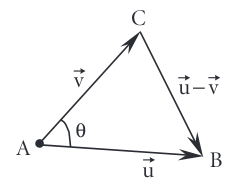
\includegraphics[width=0.6\textwidth]{./fig/fig2.1.png}
  \caption{Triângulo ABC formado pelos vetores $\vec{u}$ e $\vec{v}$}
  \label{fig:triangulo_vetores}
\end{figure}

Aplicando a lei dos cossenos ao triângulo ABC da Figura
\ref{fig:triangulo_vetores}, temos:

\begin{equation}
  \|\vec{u} - \vec{v}\|^2 = \|\vec{u}\|^2 + \|\vec{v}\|^2 - 2\|\vec{u}\|\|\vec{v}\|\cos\theta
  \label{eq:lei_cossenos}
\end{equation}

Por outro lado, de acordo com o Exemplo 2 (item anterior):

\begin{equation}
  \|\vec{u} - \vec{v}\|^2 = \|\vec{u}\|^2 + \|\vec{v}\|^2 - 2\vec{u} \cdot \vec{v}
  \label{eq:forma_algebrica}
\end{equation}

Comparando as igualdades \eqref{eq:lei_cossenos} e \eqref{eq:forma_algebrica}:

\[
  \|\vec{u}\|^2 + \|\vec{v}\|^2 - 2\vec{u} \cdot \vec{v} = \|\vec{u}\|^2 + \|\vec{v}\|^2 - 2\|\vec{u}\|\|\vec{v}\|\cos\theta
\]

Simplificando:

\[
  -2\vec{u} \cdot \vec{v} = -2\|\vec{u}\|\|\vec{v}\|\cos\theta
\]

E então:

\[
  \vec{u} \cdot \vec{v} = \|\vec{u}\| \|\vec{v}\| \cos\theta, \quad 0^\circ \leq \theta \leq 180^\circ
\]

\subsubsection*{Conclusão}
O produto escalar de dois vetores não nulos é igual ao produto de seus módulos
pelo cosseno do ângulo por eles formado.

\subsubsection*{Definição de Vetores Ortogonais}
Dois vetores $\vec{u}$ e $\vec{v}$ são \textbf{ortogonais} se, e somente se:

\begin{equation}
  \vec{u} \cdot \vec{v} = 0
  \label{eq:ortogonalidade}
\end{equation}

\begin{itemize}
  \item Pela equação \eqref{eq:produto_escalar_geometrico}, isso ocorre quando:
  \begin{itemize}
    \item $\cos\theta = 0$ (ou seja, $\theta = 90^\circ$), ou
    \item Um dos vetores é o vetor nulo $\vec{0}$
  \end{itemize}
  \item O vetor nulo é considerado ortogonal a qualquer outro vetor
  \item Notação: $\vec{u} \perp \vec{v}$ indica que $\vec{u}$ e $\vec{v}$ são ortogonais
\end{itemize}

\subsection{Cálculo do Ângulo de Dois Vetores}

Da igualdade fundamental do produto escalar:

\[
\vec{u} \cdot \vec{v} = \|\vec{u}\| \|\vec{v}\| \cos\theta
\]

Obtemos a fórmula para calcular o ângulo $\theta$ entre os vetores $\vec{u}$ e
$\vec{v}$ não nulos:

\begin{equation}
\cos\theta = \frac{\vec{u} \cdot \vec{v}}{\|\vec{u}\| \|\vec{v}\|}
\label{eq:angulo_vetores}
\end{equation}

\subsubsection*{Propriedades Importantes}

\begin{itemize}
    \item Quando $\cos\theta > 0$ (produto escalar positivo), o ângulo $\theta$ é agudo ($0^\circ \leq \theta < 90^\circ$)
    
    \item Quando $\cos\theta < 0$ (produto escalar negativo), o ângulo $\theta$ é obtuso ($90^\circ < \theta \leq 180^\circ$)
    
    \item Quando $\cos\theta = 0$ (vetores ortogonais), $\theta = 90^\circ$
    
    \item O ângulo $\theta$ é sempre o menor ângulo entre as direções dos vetores ($0^\circ \leq \theta \leq 180^\circ$)
\end{itemize}

\subsubsection*{Exemplo}

Dados os vetores $\vec{u} = (1, 2, -1)$ e $\vec{v} = (0, 1, 2)$, calcular o
ângulo entre eles:

\begin{enumerate}
  \item Cálculo do produto escalar:
  \[
  \vec{u} \cdot \vec{v} = (1)(0) + (2)(1) + (-1)(2) = 0 + 2 - 2 = 0
  \]
  
  \item Cálculo das normas:
  \[
  \|\vec{u}\| = \sqrt{1^2 + 2^2 + (-1)^2} = \sqrt{6}, \quad \|\vec{v}\| = \sqrt{0^2 + 1^2 + 2^2} = \sqrt{5}
  \]
  
  \item Aplicação da fórmula:
  \[
  \cos\theta = \frac{0}{\sqrt{6} \cdot \sqrt{5}} = 0 \Rightarrow \theta = 90^\circ
  \]
\end{enumerate}

Conclusão: Os vetores são ortogonais, como já era esperado pelo produto escalar
nulo.

\subsection{Ângulos Diretores e Cossenos Diretores de um Vetor}

Seja o vetor $\vec{v} = x\vec{i} + y\vec{j} + z\vec{k}$ não nulo.

\subsection*{Definições}
\begin{itemize}
    \item \textbf{Ângulos diretores} de $\vec{v}$ são os ângulos $\alpha$,
    $\beta$ e $\gamma$ que $\vec{v}$ forma com os vetores $\vec{i}$, $\vec{j}$ e
    $\vec{k}$, respectivamente (Figura~\ref{fig:fig2.9}).
    
    \item \textbf{Cossenos diretores} de $\vec{v}$ são os cossenos de seus
    ângulos diretores, ou seja, $\cos\alpha$, $\cos\beta$ e $\cos\gamma$.
\end{itemize}

\subsubsection*{Cálculo dos Cossenos Diretores}
Utilizando a fórmula \eqref{eq:angulo_vetores} para o ângulo entre vetores:

\begin{align}
  \cos\alpha &= \frac{\vec{v} \cdot \vec{i}}{\|\vec{v}\|\|\vec{i}\|} = \frac{(x,y,z) \cdot (1,0,0)}{\|\vec{v}\| \cdot 1} = \frac{x}{\|\vec{v}\|} \\
  \cos\beta &= \frac{\vec{v} \cdot \vec{j}}{\|\vec{v}\|\|\vec{j}\|} = \frac{(x,y,z) \cdot (0,1,0)}{\|\vec{v}\| \cdot 1} = \frac{y}{\|\vec{v}\|} \\
  \cos\gamma &= \frac{\vec{v} \cdot \vec{k}}{\|\vec{v}\|\|\vec{k}\|} = \frac{(x,y,z) \cdot (0,0,1)}{\|\vec{v}\| \cdot 1} = \frac{z}{\|\vec{v}\|}
\end{align}

\subsubsection*{Observação Importante}
Os cossenos diretores de $\vec{v}$ são precisamente as componentes do versor de
$\vec{v}$:

\[
\frac{\vec{v}}{\|\vec{v}\|} = \frac{(x,y,z)}{\|\vec{v}\|} = \left(\frac{x}{\|\vec{v}\|}, \frac{y}{\|\vec{v}\|}, \frac{z}{\|\vec{v}\|}\right) = (\cos\alpha, \cos\beta, \cos\gamma)
\]

Como o versor é um vetor unitário, decorre imediatamente que:

\begin{equation}
  \cos^2\alpha + \cos^2\beta + \cos^2\gamma = 1
  \label{eq:relacao_cossenos_diretores}
\end{equation}

\begin{figure}[h]
  \centering
  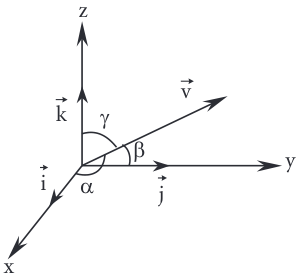
\includegraphics[width=0.5\textwidth]{./fig/fig2.9.png}
  \caption{Ângulos diretores $\alpha$, $\beta$ e $\gamma$ do vetor $\vec{v}$ em
  relação aos eixos coordenados}
  \label{fig:fig2.9}
\end{figure}

\subsection{Projeção de um Vetor Sobre Outro}

Sejam os vetores $\vec{u}$ e $\vec{v}$ não nulos e $\theta$ o ângulo entre eles.
Pretendemos decompor um dos vetores, digamos $\vec{v}$, tal que:

\[
\vec{v} = \vec{v_1} + \vec{v_2}
\]

sendo $\vec{v_1} \parallel \vec{u}$ e $\vec{v_2} \perp \vec{u}$.

\begin{figure}[H]
  \centering
  \begin{subfigure}{0.45\textwidth}
    \centering
    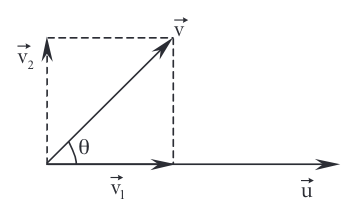
\includegraphics[width=0.6\textwidth]{./fig/fig2.10a.png}
    \caption{Ângulo agudo ($\theta < 90^\circ$)}
    \label{fig:fig2.10a}
  \end{subfigure}
  \centering
  \begin{subfigure}{0.45\textwidth}
    \centering
    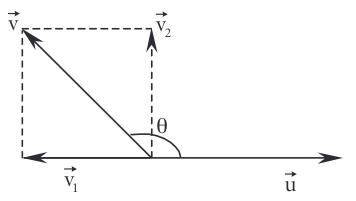
\includegraphics[width=0.6\textwidth]{./fig/fig2.10b.png}
    \caption{Ângulo obtuso ($\theta > 90^\circ$)}
    \label{fig:fig2.10b}
  \end{subfigure}
\end{figure}

O vetor $\vec{v_1}$ é chamado \textbf{projeção ortogonal} de $\vec{v}$ sobre
$\vec{u}$ e indicado por:

\begin{equation}
  \vec{v_1} = \text{proj}_{\vec{u}} \vec{v}
  \label{eq:def_projecao}
\end{equation}

Como $\vec{v_1} \parallel \vec{u}$, temos $\vec{v_1} = \alpha \vec{u}$ e como
$\vec{v_2} = \vec{v} - \vec{v_1} = \vec{v} - \alpha \vec{u}$ é ortogonal a
$\vec{u}$, vem:

\[
(\vec{v} - \alpha \vec{u}) \cdot \vec{u} = 0
\]

\[
\vec{v} \cdot \vec{u} - \alpha (\vec{u} \cdot \vec{u}) = 0
\]

\[
\alpha = \frac{\vec{v} \cdot \vec{u}}{\vec{u} \cdot \vec{u}}
\]

Portanto, sendo $\vec{v_1} = \alpha \vec{u}$, por \eqref{eq:def_projecao},
conclui-se que:

\begin{equation}
  \text{proj}_{\vec{u}} \vec{v} = \left( \frac{\vec{v} \cdot \vec{u}}{\vec{u} \cdot \vec{u}} \right) \vec{u}
  \label{eq:formula_projecao}
\end{equation}

\subsubsection*{Propriedades Importantes}
\begin{itemize}
  \item O comprimento da projeção é dado por:
  \[
  \|\text{proj}_{\vec{u}} \vec{v}\| = \frac{|\vec{v} \cdot \vec{u}|}{\|\vec{u}\|}
  \]
  
  \item Se $\vec{u}$ é unitário ($\|\vec{u}\| = 1$), a fórmula simplifica para:
  \[
  \text{proj}_{\vec{u}} \vec{v} = (\vec{v} \cdot \vec{u}) \vec{u}
  \]
  
  \item A projeção é linear:
  \[
  \text{proj}_{\vec{u}} (a\vec{v} + b\vec{w}) = a\,\text{proj}_{\vec{u}} \vec{v} + b\,\text{proj}_{\vec{u}} \vec{w}
  \]
\end{itemize}

\subsection{Interpretação Geométrica do Módulo do Produto Escalar}

Considerando a fórmula de projeção:

\[
\text{proj}_{\vec{u}} \vec{v} = \left( \frac{\vec{v} \cdot \vec{u}}{\vec{u} \cdot \vec{u}} \right) \vec{u}
\]

Quando $\vec{u}$ é unitário ($\|\vec{u}\| = 1$), temos:

\[
\vec{u} \cdot \vec{u} = \|\vec{u}\|^2 = 1
\]

Portanto, a projeção simplifica para:

\begin{equation}
\text{proj}_{\vec{u}} \vec{v} = (\vec{v} \cdot \vec{u}) \vec{u}
\label{eq:proj_vetor_unitario}
\end{equation}

Calculando o comprimento desta projeção:

\[
\|\text{proj}_{\vec{u}} \vec{v}\| = \|(\vec{v} \cdot \vec{u}) \vec{u}\| = |\vec{v} \cdot \vec{u}| \cdot \|\vec{u}\| = |\vec{v} \cdot \vec{u}|
\]

\subsubsection*{Conclusão Importante}

O comprimento da projeção ortogonal de $\vec{v}$ sobre $\vec{u}$ (quando
$\vec{u}$ é unitário) é igual ao módulo do produto escalar $\vec{v} \cdot
\vec{u}$.

\[
\|\text{proj}_{\vec{u}} \vec{v}\| = |\vec{v} \cdot \vec{u}|
\]

\subsubsection*{Interpretação Geométrica}
\begin{itemize}
  \item Quando $\theta$ é agudo ($\cos\theta > 0$), o produto escalar $\vec{v} \cdot \vec{u}$ é positivo
  \item Quando $\theta$ é obtuso ($\cos\theta < 0$), o produto escalar $\vec{v} \cdot \vec{u}$ é negativo
  \item O módulo $|\vec{v} \cdot \vec{u}|$ representa sempre o comprimento da projeção
  \item Para $\vec{u}$ não unitário, o comprimento é $\dfrac{|\vec{v} \cdot \vec{u}|}{\|\vec{u}\|}$
\end{itemize}

\subsection{Produto Escalar no Plano}

Todo o estudo feito para vetores no espaço é válido também para vetores no
plano. Considerando os vetores $\vec{u} = (x_1, y_1)$ e $\vec{v} = (x_2, y_2)$,
temos:

\subsubsection*{Propriedades no Plano}
\begin{enumerate}[label=\alph*)]
  \item Expressão do produto escalar:
  \begin{equation}
    \vec{u} \cdot \vec{v} = x_1x_2 + y_1y_2
    \label{eq:produto_plano}
  \end{equation}
  
  \item Valem todas as propriedades do produto escalar vistas anteriormente
  
  \item Ângulo entre vetores:
  \begin{equation}
    \cos\theta = \frac{\vec{u} \cdot \vec{v}}{\|\vec{u}\|\|\vec{v}\|}, \quad \text{para } \vec{u} \neq \vec{0} \text{ e } \vec{v} \neq \vec{0}
    \label{eq:angulo_plano}
  \end{equation}
  
  \item Condição de ortogonalidade:
  \begin{equation}
    \vec{u} \perp \vec{v} \iff \vec{u} \cdot \vec{v} = 0
    \label{eq:ortog_plano}
  \end{equation}
  
  \item Ângulos diretores (para $\vec{u} \neq \vec{0}$):
  \begin{align}
    \cos\alpha &= \frac{x_1}{\|\vec{u}\|} \label{eq:cos_alpha} \\
    \cos\beta &= \frac{y_1}{\|\vec{u}\|} \label{eq:cos_beta}
  \end{align}
  onde $\alpha$ e $\beta$ são os ângulos que $\vec{u}$ forma com os eixos $x$ e $y$, respectivamente
  
  \item Relação fundamental:
  \begin{equation}
    \cos^2\alpha + \cos^2\beta = 1
    \label{eq:relacao_planar}
  \end{equation}
  
  \item Projeção vetorial (para $\vec{u} \neq \vec{0}$ e $\vec{v} \neq \vec{0}$):
  \begin{equation}
    \text{proj}_{\vec{u}} \vec{v} = \left( \frac{\vec{v} \cdot \vec{u}}{\vec{u} \cdot \vec{u}} \right) \vec{u}
    \label{eq:proj_plano}
  \end{equation}
\end{enumerate}

\subsubsection*{Observações Importantes}
\begin{itemize}
    \item No plano, trabalhamos com apenas dois ângulos diretores ($\alpha$ e $\beta$)
    \item A norma de um vetor $\vec{u} = (x,y)$ é dada por $\|\vec{u}\| = \sqrt{x^2 + y^2}$
    \item A relação $\cos^2\alpha + \cos^2\beta = 1$ é o análogo bidimensional da relação tridimensional
    \item A condição de paralelismo no plano é $\frac{x_1}{x_2} = \frac{y_1}{y_2}$
\end{itemize}

\subsection{Uma Aplicação na Física}

O produto escalar é uma importante ferramenta matemática para a Física, uma vez
que inúmeras grandezas físicas são definidas com seu emprego, como, por exemplo,
o \textit{trabalho}.

\subsubsection*{Definição de Trabalho}
O trabalho realizado por uma força constante $\vec{F}$ ao longo de um
deslocamento $\vec{d}$ é definido como:

\begin{equation*}
  W = \vec{F} \cdot \vec{d}
\end{equation*}

\begin{figure}[h]
    \centering
    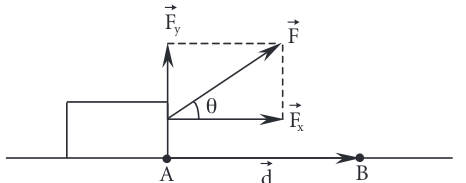
\includegraphics[width=0.5\textwidth]{./fig/fig2.12.png}
    \caption{Componente da força $\vec{F}$ na direção do deslocamento $\vec{d}$}
    \label{fig:fig2.12}
\end{figure}

\subsubsection*{Interpretação Física}
\begin{itemize}
  \item A componente efetiva da força na direção do deslocamento é:
  \[
  \|\vec{F_x}\| = \|\vec{F}\| \cos\theta
  \]
  onde $\theta$ é o ângulo entre a força e o deslocamento
  
  \item O trabalho é uma grandeza \textbf{escalar}
  
  \item Unidade no SI: joule (J), onde $1\,\text{J} = 1\,\text{N} \cdot \text{m}$
\end{itemize}

\subsubsection*{Expressões Equivalentes}
O trabalho pode ser calculado por:

\begin{equation*}
  W = \|\vec{F}\| \|\vec{d}\| \cos\theta
\end{equation*}

ou, em termos das componentes:

\[
W = F_x d_x + F_y d_y + F_z d_z \quad \text{(em 3D)}
\]

\subsubsection*{Casos Particulares}
\begin{itemize}
  \item Quando $\theta = 0^\circ$ (força paralela ao deslocamento):
  \[
  W = \|\vec{F}\| \|\vec{d}\| \quad \text{(trabalho máximo)}
  \]
  
  \item Quando $\theta = 90^\circ$ (força perpendicular ao deslocamento):
  \[
  W = 0
  \]
  
  \item Quando $180^\circ > \theta > 90^\circ$:
  \[
  W < 0 \quad \text{(trabalho resistivo)}
  \]
\end{itemize}
